\chapter{Background \& Objectives}

This project addresses the challenge of enabling autonomous navigation for an F1Tenth racing car using the DreamerV3 reinforcement learning framework and LiDAR data. DreamerV3, a model-based reinforcement learning algorithm, has demonstrated impressive performance in various domains, but its typical use with image-based inputs presents a significant hurdle when dealing with the LiDAR range data provided by the F1Tenth's primary sensor. Our work is motivated by the need for robust and efficient autonomous racing solutions on resource-constrained platforms where image processing may be computationally expensive or impractical.

\section{Background}
\begin{itemize}
    \item DreamerV3 and MBRL: Studied DreamerV3 architecture, training, and performance. Researched model-based RL principles and related algorithms.
    \item F1Tenth and ROS2: Investigated F1Tenth platform, ROS2, message types, and external simulations. Explored existing F1Tenth projects.
    \item Existing Implementations: Analyzed DreamerV3 code repositories and similar projects using image-based inputs or other robotic platforms. Researched data representation for neural networks.
    \item Motivation: Driven by interest in robotics and AI, particularly autonomous racing challenges. Motivated to adapt DreamerV3 to LiDAR inputs and contribute to efficient autonomous racing solutions.
\end{itemize}

\section{Analysis}
Our background research revealed that directly applying DreamerV3 to the F1Tenth platform with its 1D LiDAR input presents two key challenges.  First, DreamerV3's world model is designed to process image-like data through convolutional neural networks (CNNs), making it incompatible with the 1D range data from the LiDAR. Second, the real-time requirements of autonomous racing necessitate an efficient integration with the ROS2-based F1Tenth simulator.

\newpage

Our analysis of these challenges led us to decompose the problem into four main tasks:
\begin{itemize}
    \item \textbf{LiDAR Data Adaptation}:  We needed to bridge the gap between the 1D LiDAR data and DreamerV3's input requirements.  Two primary approaches emerged:
    \begin{itemize}
        \item \textbf{Image-like Conversion}: Transforming the 1D range data into a 2D representation resembling an image, suitable for input to a CNN. This could involve polar coordinate transformations or creating a simple occupancy grid.
        \item \textbf{MLP-based Adaptation}: Modifying DreamerV3's world model to directly accept 1D input using a multi-layer perceptron (MLP) instead of a CNN.
    \end{itemize}
    \item \textbf{Custom Environment Development}:  A custom Gymnasium environment was required to provide a standardized interface between DreamerV3 and external gym simulators.  This environment would handle data transfer, reward calculation, and interaction with the simulated car.
    \item \textbf{Training Simulation}: Either through a multi-core training environment or any other training options, we aim to create reliable software to train our model that maximizes computational efficiency.
    \item \textbf{ROS2 Integration}:  Seamless integration with the ROS2 framework is crucial for real-time control. This involves establishing communication channels between DreamerV3 and the simulator using ROS2 topics and messages.
\end{itemize}

\begin{figure}
    \centering
    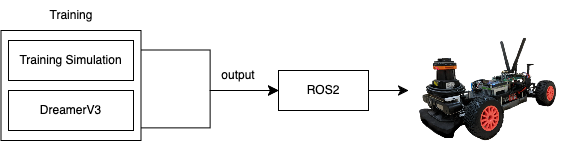
\includegraphics[scale=0.65]{deploy}
    \caption{Deployment stages}
    \label{fig:deploy}
\end{figure}

Our core objective is to pursue either the image-like conversion and the MLP-based adaptation approaches based on efficient code structures, or attempt to convert the sensor data into an image-based observation.  While the image-like conversion offers the advantage of leveraging DreamerV3's existing CNN architecture, we recognize that it might introduce information loss or require complex transformations. The MLP-based adaptation, while requiring more extensive code modifications, offers the potential for more direct and efficient processing of the LiDAR data \ref{fig:deploy}.

\section{Process}
This project follows an iterative and incremental development process, adapted from the agile methodology.  While a full-fledged agile framework with sprints and formal reviews isn't strictly necessary for this project's scale, the core principles of iterative development, continuous integration, and close collaboration seem fitting.  Our plan can be broken down into the following phases :

\begin{figure}
    \centering
    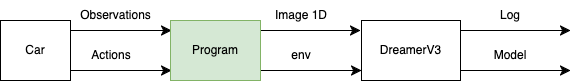
\includegraphics[scale=0.6]{program}
    \caption{Program schema}
    \label{fig:program}
\end{figure}

\begin{itemize}
    \item[1.] \textbf{Planning and Requirements Gathering (Initial Phase)}:  This initial phase involved defining the project scope, identifying key objectives, and analyzing the technical requirements.  We conducted background research, explored existing implementations, and analyzed the F1Tenth platform and its ROS2 environment \ref{fig:program}.

    \item[2.] \textbf{Design and Implementation (Iterative Cycles)}: This phase forms the core of our development process.  We adopt an iterative approach, focusing on developing and testing individual components before integrating them into the larger system.  Each iteration typically involves:
    \begin{itemize}
        \item \textbf{Component Development:} Implementing a specific module, such as the custom Gymnasium environment, the data preprocessing module, or a modification to the DreamerV3 codebase.
        \item \textbf{Unit Testing:} Thoroughly testing each component in isolation to ensure its functionality and identify potential bugs early on.
        \item \textbf{Integration:} Integrating the developed component with the existing system.
        \item \textbf{System Testing:} Testing the integrated system to ensure that the components work together correctly.
    \end{itemize}
    
    \item[3.] \textbf{Testing and Evaluation (Continuous)}: Testing is an ongoing process throughout the project.  We employ unit tests for individual components and system tests for integrated modules.  As the project progresses, we will conduct more extensive testing in the simulated F1Tenth environment to evaluate the performance of the trained agents.  This continuous testing allows us to identify and address issues early in the development cycle.
    
    \item[4.] \textbf{Documentation and Reporting (Ongoing)}: Documentation will be maintained throughout the project, with regular updates to this document, code comments, and a final project report.  This ensures that the project's progress, design decisions, and implementation details are clearly recorded.
\end{itemize}
This iterative and incremental process will provide high efficiency for this project.  It allows us to break down the complex task of integrating DreamerV3 with the F1Tenth platform into smaller, manageable units.  The continuous testing and integration enables us to identify and address issues early, preventing them from escalating into larger problems later on.  The flexibility of this approach also allows us to adapt to unforeseen challenges and adjust our plans as needed.
